\section{GDB：让程序停下来看看}

\begin{frame}{GDB是什么？}
    \alert{GDB（GNU Debugger）}是GNU项目的调试器，本课使用它调试C语言编写的程序。
    \medskip
    \begin{itemize}
        \item \alert{启动程序}：指定参数和输入，复现出错的运行过程。
        \item \alert{暂停执行}：在某个位置、条件成立或变量改变时停下来。
        \item \alert{查看现场}：观察变量、源码位置和函数调用关系。
        \item \alert{控制执行}：逐步运行，找到实际行为第一次偏离预期的位置。
    \end{itemize}
    \medskip
    \begin{vspquotered}{从源码到调试}
        \texttt{gcc}将C源码编译为可执行程序；GDB加载并调试这个程序。\par
        VSCode可以通过扩展调用编译器与调试器，提供图形化操作界面。
    \end{vspquotered}
    \small 调试信息帮助GDB显示源码行号与变量；后面将介绍编译参数\texttt{-g}。
\end{frame}

\begin{frame}{GDB与GCC有什么区别？}
    \alert{GCC负责把源码编译成程序，GDB负责观察和控制程序的运行。}
    \medskip
    \begin{columns}[T]
        \begin{column}{0.51\textwidth}
            \small
            \begin{itemize}
                \item \texttt{gcc}读取C源码，编译、链接成可执行程序。
                \item \texttt{gdb}加载可执行程序，设置断点、查看变量、单步执行。
            \end{itemize}
            \medskip
            在终端中\alert{先编译，再启动调试}：
            \lstset{basicstyle=\ttfamily\fontsize{7.2}{8.7}\selectfont,
                numberstyle=\fontsize{4.8}{5.5}\selectfont\color{gray},
                xleftmargin=6pt,breakatwhitespace=true}
            \begin{Code}*{bash}
                \lstinputlisting{code/commands/compile-and-debug.sh}
            \end{Code}
            修改源码后，需要先重新编译。
        \end{column}
        \begin{column}{0.45\textwidth}
            \small
            \renewcommand{\arraystretch}{1.25}
            \begin{tabular}{@{}p{0.27\linewidth}p{0.65\linewidth}@{}}
                \textbf{选项} & \textbf{含义} \\
                \texttt{-g} & 生成调试信息，便于GDB定位源码和变量。 \\
                \texttt{-O0} & 关闭优化，便于逐行调试。 \\
                \texttt{-Wall} & 开启一组常用编译警告。 \\
                \texttt{-Wextra} & 开启额外的编译警告。 \\
                \texttt{-Wpedantic} & 提示部分不符合所选ISO C标准的写法。 \\
                \texttt{-Werror} & 将警告视为错误，有警告时编译失败。
            \end{tabular}
        \end{column}
    \end{columns}
    \medskip
    \footnotesize \texttt{-O0}中的O是字母、0是数字；\texttt{-Wall}并非开启全部警告。
    \note{补充六个GCC选项的含义。-g生成调试信息；-O0便于本课按源码逐行观察。-Wall与-Wextra启用不同的警告集合，-Wpedantic依据-std=c17检查部分标准符合性，-Werror将警告提升为错误。提醒不要将-Werror拼成-Werro。}
\end{frame}

\begin{frame}{安装GDB：Ubuntu／WSL}
    在\alert{Ubuntu／WSL的Ubuntu终端}执行以下命令，需要当前账号拥有sudo权限：
    \begin{Code}*{bash}
        \lstinputlisting{code/commands/install.sh}
    \end{Code}
    \begin{columns}[c]
        \begin{column}{0.62\textwidth}
            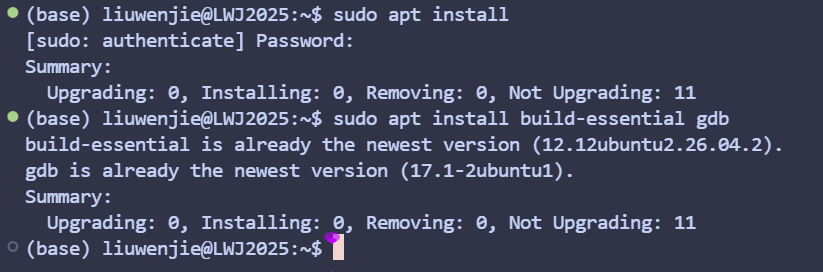
\includegraphics[width=\linewidth,height=0.40\textheight,keepaspectratio]{gdb_install.png}
        \end{column}
        \begin{column}{0.34\textwidth}
            \small
            \begin{itemize}
                \item \texttt{apt update}：更新软件包索引。
                \item \texttt{build-essential}：GCC、Make等构建工具。
                \item \texttt{gdb}：GDB调试器。
            \end{itemize}
        \end{column}
    \end{columns}
    \medskip
    \small 截图中的\texttt{is already the newest version}表示相应工具已安装。
    \par 共享服务器可能使用其他发行版或没有sudo权限，安装前先确认环境。
    \note{展示用户提供的image/gdb_install.png。截图显示build-essential与gdb已为该环境中的最新可用版本；版本号以实际环境为准。Windows用户先进入WSL的Ubuntu环境。}
\end{frame}

\begin{frame}{没有sudo权限时怎么使用GDB？}
    \texttt{is not in the sudoers file}表示当前账号没有sudo权限。
    \begin{itemize}
        \item 在共享服务器上，使用管理员提供的工具，或已准备好的用户目录工具。
        \item 本项目当前演示机是\alert{RHEL 8.10}；Ubuntu的\texttt{apt}安装命令不适用。
    \end{itemize}
    \medskip
    当前工作区已准备好本地GDB与运行库，可以在Bash中执行：
    \begin{Code}*{bash}
        \lstinputlisting{code/commands/use-local-tools.sh}
    \end{Code}
    \small 这里加载的是本工作区已有工具。每次打开新终端需重新加载；清理\texttt{build/}后需重新准备这些工具。其他服务器的工具路径以管理员说明为准。
\end{frame}

\begin{frame}{安装完成后，如何验证？}
    \begin{columns}[T]
        \begin{column}{0.48\textwidth}
            在\alert{终端}中依次执行：
            \begin{Code}*{bash}
                \lstinputlisting{code/commands/verify-install.sh}
            \end{Code}
            \texttt{command -v}显示GDB路径；\par
            \texttt{--version}显示版本信息。
        \end{column}
        \begin{column}{0.48\textwidth}
            出现\alert{\texttt{(gdb)}}提示符后输入：
            \begin{Code}*{plain}
                \lstinputlisting{code/commands/verify-install.gdb}
            \end{Code}
            \texttt{help}显示命令帮助；\par
            \texttt{quit}退出并回到终端。
        \end{column}
    \end{columns}
    \medskip
    \begin{vspquotered}{验证成功的标志}
        能找到路径、显示版本，并进入GDB执行\texttt{help}，说明工具已可启动。\par
        若提示\texttt{command not found}，先检查安装位置或是否加载了本地工具环境。
    \end{vspquotered}
\end{frame}

\begin{frame}{这四行命令分别验证什么？}
    \begin{center}
        \renewcommand{\arraystretch}{1.3}
        \begin{tabular}{p{0.25\linewidth}p{0.65\linewidth}}
            \textbf{终端命令} & \textbf{含义与成功时的现象} \\
            \texttt{command -v gdb} &
                让Shell查找\texttt{gdb}命令，检查当前终端能否找到它；通常输出可执行文件路径。 \\
            \texttt{gdb --version} &
                显示GDB的版本信息并退出，确认调试器可以运行，也方便记录调试环境。 \\
            \texttt{gcc --version} &
                显示GCC的版本信息并退出，确认C编译器可以运行；后面用它编译示例源码。 \\
            \texttt{gdb -q} &
                以安静模式启动GDB，省略欢迎语和版权信息；出现\texttt{(gdb)}后即可输入调试命令。
        \end{tabular}
    \end{center}
    \medskip
    \texttt{-q}中的q表示\alert{quiet}；进入GDB后用\texttt{help}查看帮助，用\texttt{quit}退出。
    \par\small 工具已经安装但终端找不到时，检查\texttt{PATH}，或重新加载本地工具环境。
\end{frame}

\begin{frame}{安装验证：路径、版本与交互界面}
    \begin{columns}[T]
        \begin{column}{0.48\textwidth}
            \alert{查找路径、查看版本}
            \par\medskip
            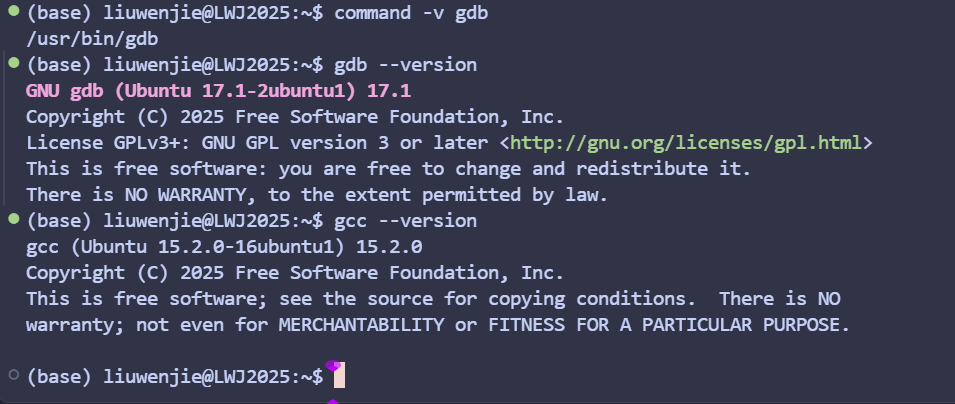
\includegraphics[width=\linewidth,height=0.64\textheight,keepaspectratio]{gdb_version.png}
            \par\medskip
            \small 显示GDB路径，以及GDB、GCC的版本信息。
        \end{column}
        \begin{column}{0.48\textwidth}
            \alert{启动GDB、查看帮助、退出}
            \par\medskip
            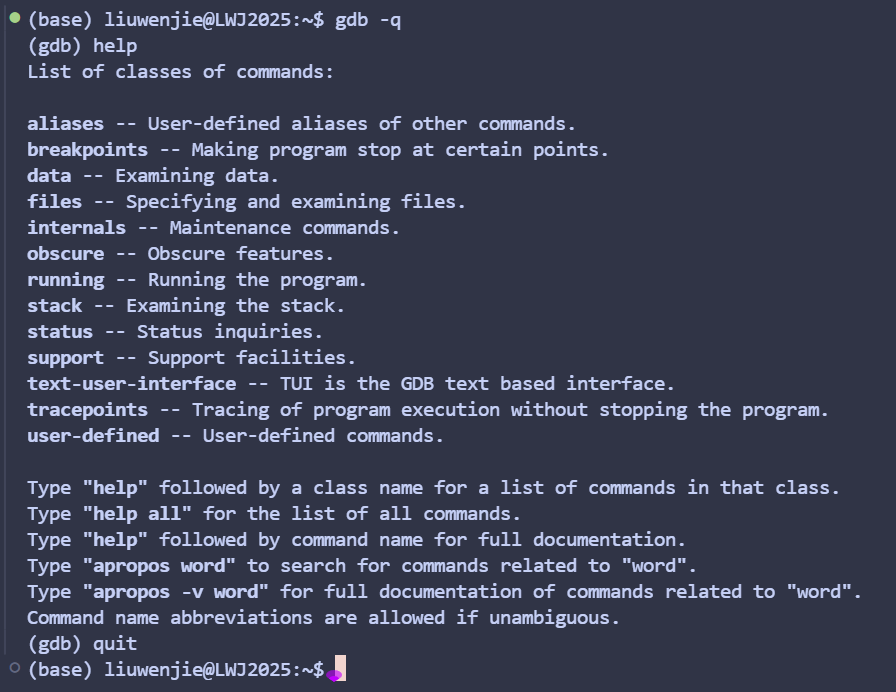
\includegraphics[width=\linewidth,height=0.64\textheight,keepaspectratio]{gdb-q.png}
            \par\small \texttt{gdb -q}进入，\texttt{help}查看帮助，\texttt{quit}退出。
        \end{column}
    \end{columns}
    \note{使用用户提供的image/gdb_version.png与image/gdb-q.png，分别展示前三条安装验证命令的输出和第四条命令的交互过程。版本号与路径取决于实际安装环境，不要求与截图一致。}
\end{frame}

\begin{frame}{GDB常用命令速查}
    \begin{center}
        \renewcommand{\arraystretch}{1.0}
        \begin{tabular}{lll}
            \textbf{命令示例} & \textbf{常用缩写} & \textbf{作用} \\
            \texttt{run} & \texttt{r} & 启动或重新运行程序 \\
            \texttt{break main} & \texttt{b main} & 在main函数设置断点 \\
            \texttt{continue} & \texttt{c} & 继续运行 \\
            \texttt{next} & \texttt{n} & 在当前调用层级单步执行 \\
            \texttt{step} & \texttt{s} & 单步执行，尝试进入函数 \\
            \texttt{finish} & \texttt{fin} & 运行到当前选定函数返回 \\
            \texttt{print value} & \texttt{p value} & 查看变量或表达式的值 \\
            \texttt{list} & \texttt{l} & 查看源码 \\
            \texttt{backtrace} & \texttt{bt} & 查看调用栈 \\
            \texttt{help break} & \texttt{h break} & 查看某条命令的帮助 \\
            \texttt{quit} & \texttt{q} & 退出GDB
        \end{tabular}
    \end{center}
    \small 这些命令在\texttt{(gdb)}中输入；终端中的\texttt{gdb ./程序}用于启动调试器。
\end{frame}

\begin{frame}{让编译结果适合调试}
    \begin{Code}*{bash}
        \lstinputlisting{code/commands/build-debug.sh}
    \end{Code}
    \begin{itemize}
        \item \texttt{-std=c17}：显式指定本课使用的C17语言标准。
        \item \texttt{-g}：加入调试信息；\texttt{-O0}：本次演示关闭优化，便于逐行观察。
        \item \texttt{-Wall -Wextra -Wpedantic}：开启常用编译警告。
        \item 修改源码后\alert{重新编译}，确认正在调试的是新生成的程序。
    \end{itemize}
    \small 优化会改变源码与机器指令的对应关系；出现\texttt{optimized out}时检查构建参数。
\end{frame}

\begin{frame}{HW1：先看调用者与辅助函数}
    \begin{columns}[T]
        \begin{column}{0.52\textwidth}
            \alert{主循环中的调用：}
            \begin{Code}*{c}
                \lstinputlisting[firstline=18,lastline=24,firstnumber=18]{code/homework/hw1-p3.c}
            \end{Code}
        \end{column}
        \begin{column}{0.44\textwidth}
            \alert{更新最大值：}
            \begin{Code}*{c}
                \lstinputlisting[firstline=4,lastline=10,firstnumber=4]{code/homework/hw1-p3.c}
            \end{Code}
        \end{column}
    \end{columns}
    \medskip
    处理输入5时，\texttt{x == 5}、\texttt{sum == 8}。\par
    \alert{传入辅助函数的value应该是多少？实际又是多少？}
\end{frame}

\begin{frame}{先把失败输入固定下来}
    \begin{itemize}
        \item 输入文件：\texttt{code/input/sum-max.txt}，内容为\texttt{3 5 2 0}。
        \item 正常运行：\texttt{./build/demo/hw1-p3 < code/input/sum-max.txt}。
        \item 预期\texttt{10 5}，实际\texttt{10 10}；保留这个反例。
    \end{itemize}
    \medskip
    \begin{vspquotered}{下一步要验证的猜想}
        总和正确，但更新最大值时可能比较了错误的数据。\par
        观察调用者的\texttt{x / sum}与被调用函数的\texttt{value / result}。
    \end{vspquotered}
    \medskip
    \alert{小输入可以手算，也方便逐步跟踪。}
\end{frame}

\begin{frame}{第一次启动GDB}
    在终端启动调试器：
    \begin{Code}*{bash}
        \lstinputlisting{code/commands/start-gdb.sh}
    \end{Code}
    进入\texttt{(gdb)}提示符后输入：
    \begin{Code}*{plain}
        \lstinputlisting[firstline=1,lastline=2,firstnumber=1]{code/commands/basic.gdb}
    \end{Code}
    \begin{itemize}
        \item \texttt{break updateMaximum}：在更新最大值的函数设置断点。
        \item \texttt{run < ...}：使用同一份输入启动程序。
        \item 程序停住后，GDB显示当前源码位置。
    \end{itemize}
\end{frame}

\begin{frame}{HW1：从断点现场定位传参错误}
    \begin{columns}[c]
        \begin{column}{0.54\textwidth}
            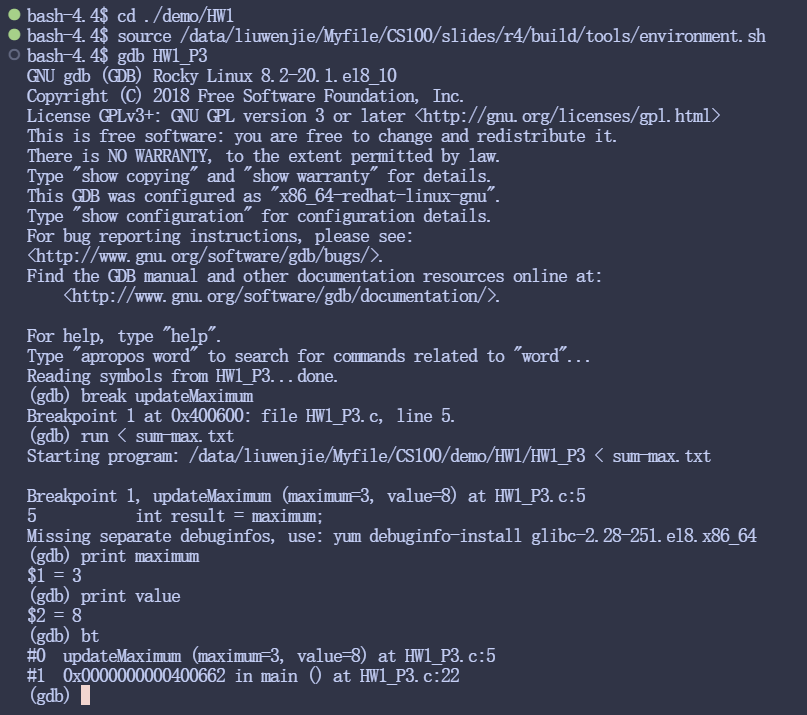
\includegraphics[width=\linewidth,height=0.80\textheight,keepaspectratio]{HW1_P3GDB.png}
        \end{column}
        \begin{column}{0.42\textwidth}
            \small
            \alert{断点已命中，检查传入的数据}
            \begin{itemize}
                \item \texttt{maximum = 3}：此前读到的最大值，符合预期。
                \item \texttt{value = 8}：当前输入是5，函数却收到了累计总和$3+5=8$。
                \item \texttt{bt}：当前在\texttt{updateMaximum}，调用来自\texttt{main}第22行。
            \end{itemize}
            \medskip
            \alert{检查调用处：将sum改为x}
            \par\texttt{updateMaximum(maximum, x)}
            \medskip

            \footnotesize 当前停在第5行，\texttt{result}尚未初始化；先执行\texttt{next}再查看它。
        \end{column}
    \end{columns}
    \note{截图使用image/HW1_P3GDB.png。第一次调用发生在读入5之后，maximum=3、sum=8；截图直接显示传入value=8，bt给出main第22行这一调用位置。可进一步frame 1、print x、print sum验证，再修复调用并重新编译，输入3 5 2 0应输出10 5。截图的系统库debuginfo提示不妨碍本例查看自己的源码和变量。}
\end{frame}

\begin{frame}{断点：只在你关心的位置停下来}
    \begin{center}
        \renewcommand{\arraystretch}{1.35}
        \begin{tabular}{ll}
            \textbf{命令} & \textbf{作用} \\
            \texttt{break updateMaximum} & 在函数入口设置断点 \\
            \texttt{break code/homework/hw1-p3.c:22} & 在指定文件行设置断点 \\
            \texttt{info breakpoints} & 查看断点编号与位置 \\
            \texttt{disable 1} / \texttt{enable 1} & 禁用／启用编号1的断点 \\
            \texttt{delete 1} & 删除编号1的断点 \\
            \texttt{continue} & 继续执行，直到再次停止
        \end{tabular}
    \end{center}
    \medskip
    \alert{当前行通常是即将执行的源码行。}读取变量时，要留意该行是否已经执行。
\end{frame}

\begin{frame}{观察变量：实际值符合预期吗？}
    在辅助函数中、\texttt{result}初始化后停住，再使用：
    \begin{Code}*{plain}
        \lstinputlisting{code/commands/inspect.gdb}
    \end{Code}
    \begin{columns}[c]
        \begin{column}{0.65\textwidth}
            \begin{itemize}
                \item \texttt{print}（\texttt{p}）：这一次查看一个变量或表达式。
                \item \texttt{display}：以后每次停止时自动显示表达式。
                \item \texttt{info locals}：查看当前栈帧中的局部变量。
            \end{itemize}
        \end{column}
        \begin{column}{0.29\textwidth}
            \centering
            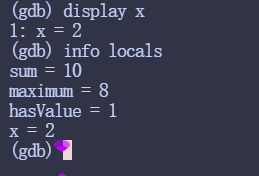
\includegraphics[width=\linewidth,height=0.30\textheight,keepaspectratio]{info.png}
            \par\scriptsize 截图：\texttt{main}中的局部变量。
        \end{column}
    \end{columns}
    \medskip
    变量存在\alert{作用域}；查看调用者的\texttt{x}和\texttt{sum}时，先切换到对应栈帧。
    \note{右侧使用image/info.png，展示main中display x与info locals的输出。截图属于第三个输入2的现场，x=2、sum=10、maximum=8；与上方辅助函数中的result示例处于不同的栈帧。}
\end{frame}

\begin{frame}{next、step与finish：函数调用处怎么走？}
    \begin{center}
        \begin{tikzpicture}[>=Stealth,node distance=0.9cm,
            box/.style={draw=VSPPrimary,rounded corners,align=left,
            inner sep=7pt,font=\small\ttfamily}]
            \node[box] (main) {main()\\\quad updateMaximum(maximum, sum);\\\quad print result;};
            \node[box,right=of main] (fn) {updateMaximum()\\\quad compare value;\\\quad return result;};
            \draw[->,thick] (main.north east) to[bend left=15]
                node[above,font=\small] {step：进入函数} (fn.north west);
            \draw[->,thick] (fn.south west) to[bend left=15]
                node[below,font=\small] {finish：运行至返回} (main.south east);
        \end{tikzpicture}
    \end{center}
    \begin{itemize}
        \item \texttt{next}（\texttt{n}）：在当前调用层级向前走，通常跨过函数调用。
        \item \texttt{step}（\texttt{s}）：尝试进入有源码调试信息的被调用函数。
        \item \texttt{finish}：运行到当前选定函数返回之后。
    \end{itemize}
    \small 遇到断点或信号可能提前停止。进入标准库内部时，可用\texttt{finish}返回。
\end{frame}

\begin{frame}{HW1现场：step、next与finish分别做了什么？}
    \begin{columns}[c]
        \begin{column}{0.54\textwidth}
            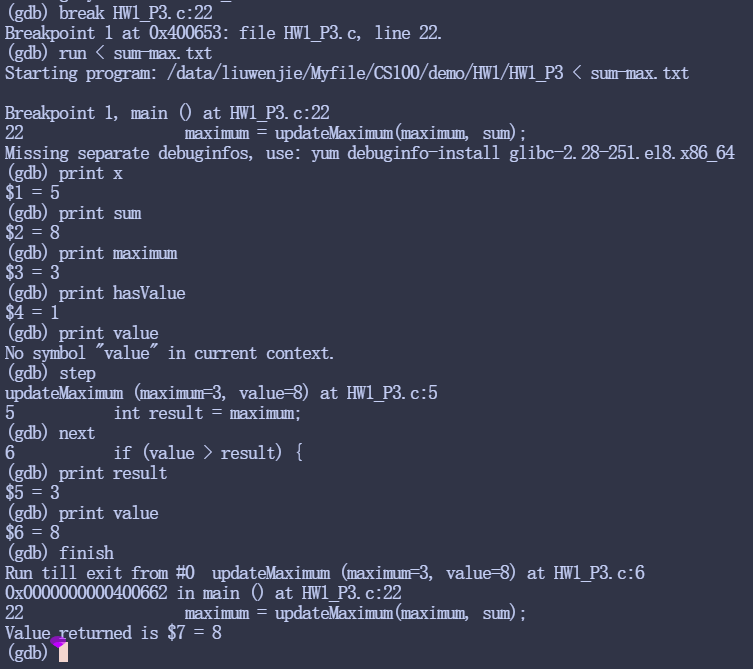
\includegraphics[width=\linewidth,height=0.80\textheight,keepaspectratio]{step_next_finish.png}
        \end{column}
        \begin{column}{0.42\textwidth}
            \small
            \begin{enumerate}
                \item \alert{step：进入函数。}\par
                    从\texttt{main}第22行进入\texttt{updateMaximum}第5行，收到\texttt{maximum=3, value=8}。
                \item \alert{next：执行初始化。}\par
                    执行第5行后停在第6行；此时\texttt{result=3}，\texttt{value=8}。
                \item \alert{finish：运行到函数返回。}\par
                    执行后续比较与返回，回到\texttt{main}，显示返回值\alert{8}。
            \end{enumerate}
            \medskip
            \footnotesize 若在第22行直接用\texttt{next}，则跨过这次调用。截图中\texttt{finish}后仍显示第22行，可再\texttt{next}完成赋值并查看\texttt{maximum}。
            \par\medskip
            \texttt{value}是辅助函数的形参，在\texttt{main}中不可直接查看。
        \end{column}
    \end{columns}
    \note{使用image/step_next_finish.png。截图在第二个输入5时停止，main中x=5、sum=8、maximum=3；step进入函数后，next执行result的初始化，再finish执行函数剩余部分并显示返回值8。finish可能停在调用行的赋值完成之前，应再next并print maximum确认。错误仍是将sum传入，应改传x；修复后这次调用应返回5。}
\end{frame}

\begin{frame}{调用栈：是谁走到了这里？}
    \begin{columns}[T]
        \begin{column}{0.43\textwidth}
            \begin{Code}*{plain}
                \lstinputlisting{code/commands/stack.gdb}
            \end{Code}
        \end{column}
        \begin{column}{0.53\textwidth}
            \begin{tikzpicture}[every node/.style={draw=VSPPrimary,
                minimum width=4.6cm,minimum height=0.9cm,align=center},node distance=0.25cm]
                \node (top) {\texttt{\#0 updateMaximum(3, 8)}\\当前函数};
                \node[below=of top] {\texttt{\#1 main()}\\它的调用者};
            \end{tikzpicture}
        \end{column}
    \end{columns}
    \medskip
    \begin{itemize}
        \item \texttt{bt}：列出调用栈；\texttt{frame 1}：选中调用者的栈帧。
        \item 切换栈帧会改变你正在观察的局部变量上下文。
        \item \alert{切换栈帧是在查看现场，不会让程序倒退执行。}
    \end{itemize}
\end{frame}

\begin{frame}{崩溃或卡住时，也能查看现场}
    \begin{itemize}
        \item 程序收到\texttt{SIGSEGV}等信号时，GDB通常会停止。
        \item 使用\texttt{bt}查看调用链，再用\texttt{frame}、\texttt{print}检查参数与局部变量。
        \item 程序持续运行时，在GDB终端按\texttt{Ctrl+C}中断，再查看当前位置。
        \item 判断它是在等待输入、重复执行循环，还是停留在某次调用中。
    \end{itemize}
    \medskip
    \begin{vspquotered}{崩溃位置是一条线索}
        如果停在标准库内部，沿调用栈找到自己的代码，检查传入的数据。\par
        内存可能在更早的时候被破坏；结合Sanitizer继续追查。
    \end{vspquotered}
\end{frame}

\begin{frame}{条件断点：只观察传入8的这次调用}
    \begin{Code}*{plain}
        \lstinputlisting{code/commands/condition.gdb}
    \end{Code}
    \begin{itemize}
        \item 处理第二个输入5时，总和已经变为8；断点匹配\texttt{value == 8}。
        \item \texttt{next}执行初始化后，局部\texttt{result == 3}，实参\texttt{value == 8}。
        \item 用\texttt{bt}和\texttt{frame 1}回看调用者：\alert{当前输入x明明是5}。
    \end{itemize}
    \small 条件表达式要使用断点位置可见的变量；重新演示前可删除旧断点。
\end{frame}

\begin{frame}{观察点：这个变量什么时候变了？}
    在\texttt{updateMaximum}中、\texttt{result}初始化为3后设置：
    \begin{Code}*{plain}
        \lstinputlisting{code/commands/watch.gdb}
    \end{Code}
    \begin{itemize}
        \item \texttt{watch result}：值改变时停止，并显示新旧值。
        \item 单步执行比较与赋值，观察\texttt{result}从3变为8。
        \item 函数正确比较了它收到的两个数；\alert{调用者却传入了sum而不是x}。
    \end{itemize}
    \medskip
    \small 局部变量离开作用域后，相关观察点可能被删除；硬件观察点资源也有限。
\end{frame}

\begin{frame}{现场演示一：找到第一次偏离预期的状态}
    \begin{enumerate}
        \item 运行HW1课堂变体，确认\texttt{3 5 2 0}输出\texttt{10 10}。
        \item 在\texttt{updateMaximum}设置\texttt{value == 8}的条件断点。
        \item 对照调用栈：调用者的\texttt{x == 5}，函数收到的却是\texttt{value == 8}。
        \item 单步和观察点确认：这次调用把最大值从3更新为8。
        \item 把调用的第二个参数由\texttt{sum}改为\texttt{x}，重新编译。
        \item 重跑反例，再检查单个数据、重复最大值与0结束标记。
    \end{enumerate}
    \medskip
    \alert{函数内部没有写错，也可能因为调用者传错参数而得到错误结果。}
    \note{本节约30分钟，含8至10分钟演示。完整批处理在code/commands/session.gdb；修复版为code/fixed/hw1-p3.c。}
\end{frame}
